\section{Performantie}
\label{sec:evaluatie-performantie}

%%%%%%%%%%%%

% Overzichtsgrafiek

% Volgens de POC is Lungo de winnaar, maar aangezien er niet alles is geïmplementeerd zou je kunnen denken dat daarom is, maar het duidelijkst is bij de loginschermen, alle 3 zijn quasi hetzelfde, behalve Lungo is een halvering van de tijd
% De tweede plaats gaat naar jQM, volgend door Kendo en als laatste ST
% De cache factor van ST is constant (gemiddeld 1,8)
% De andere raamwerken hebben een beduidend grotere cache factor 

% TODO Tim: tabel maken voor de dingen hieronder
% deze dingen uitdiepen hieronder
% page speed
% LOC
% download grootte
% subjectieve experience lijsten

\begin{figure}
  \centering
  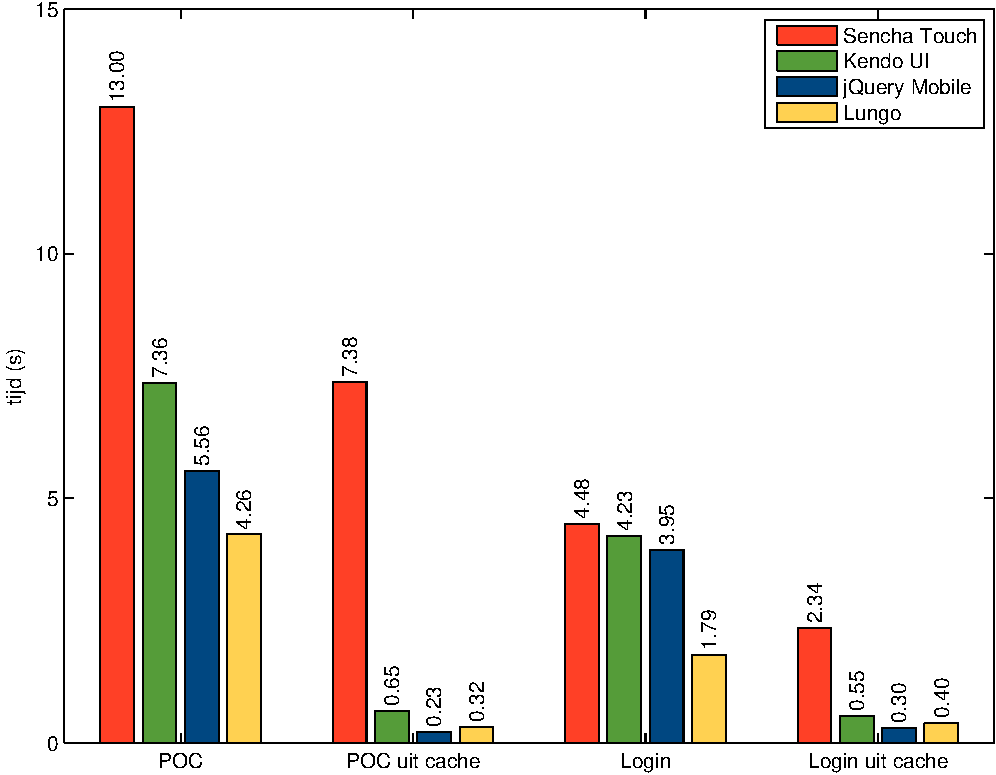
\includegraphics[width=0.8\textwidth]{figuren/performance.pdf}
  \caption{Downloadtijden voor POC,  POC uit cache,  Login en Login uit cache voor elk raamwerk.}
  \label{fig:performantie}
\end{figure}


\subsection{\st}

\begin{figure}
  \centering
  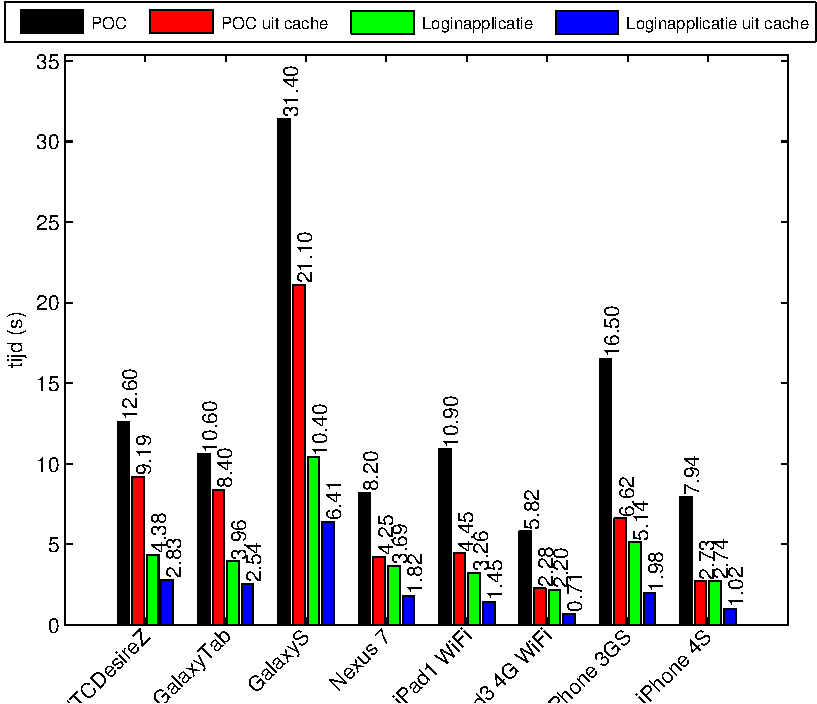
\includegraphics[width=0.5\textwidth]{figuren/performance-st.pdf}
  \caption{Downloadtijden van \st{} voor POC,  POC uit cache,  Login en Login uit cache voor elk device.}
  \label{fig:performantie-st}
\end{figure}

\subsection{\kendo}

\begin{figure}
  \centering
  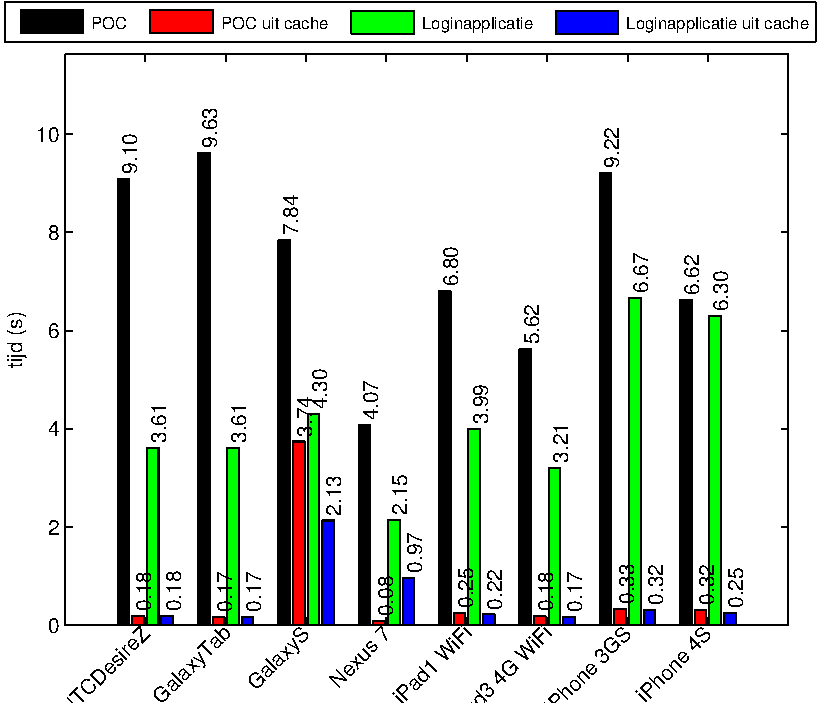
\includegraphics[width=0.5\textwidth]{figuren/performance-kendo.pdf}
  \caption{Downloadtijden van \kendo{} voor POC,  POC uit cache,  Login en Login uit cache voor elk device.}
  \label{fig:performantie-kendo}
\end{figure}

\subsection{\jqm}

\begin{figure}
  \centering
  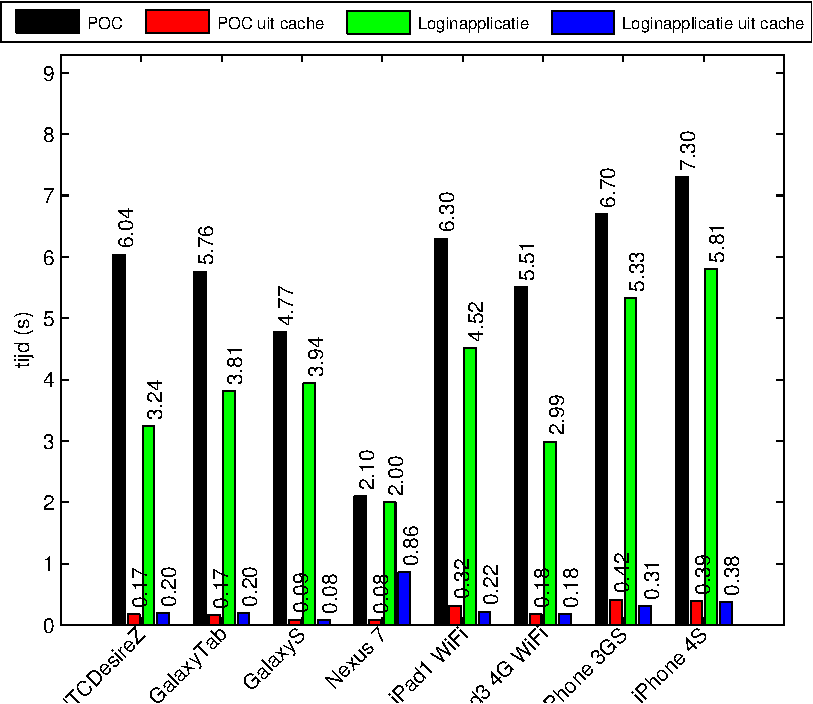
\includegraphics[width=0.5\textwidth]{figuren/performance-jquery.pdf}
  \caption{Downloadtijden van \jqm{} voor POC,  POC uit cache,  Login en Login uit cache voor elk device.}
  \label{fig:performantie-jqm}
\end{figure}

\subsection{\lungo}

\begin{figure}
  \centering
  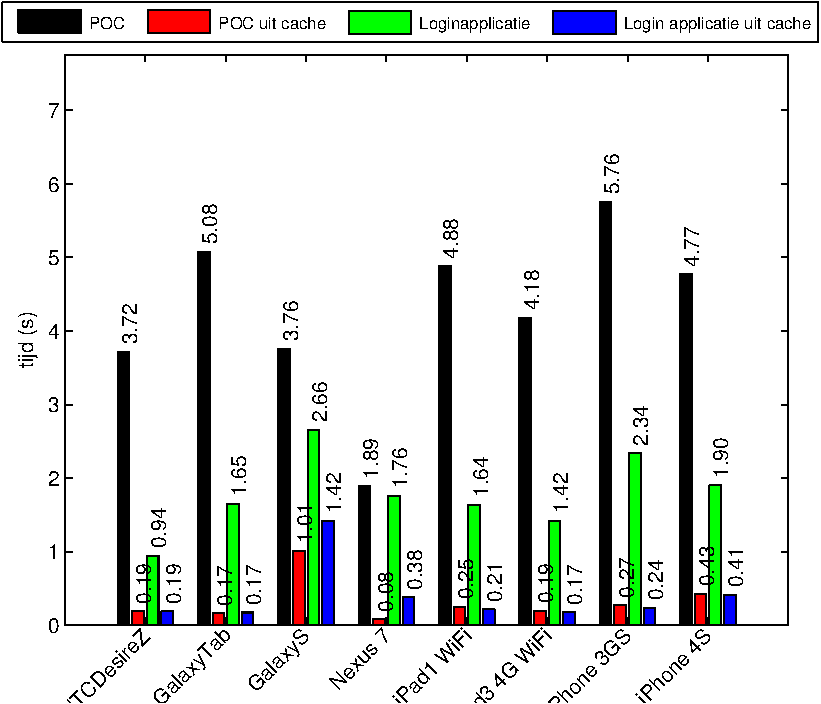
\includegraphics[width=0.5\textwidth]{figuren/performance-lungo.pdf}
  \caption{Downloadtijden van \lungo{} voor POC,  POC uit cache,  Login en Login uit cache voor elk device.}
  \label{fig:performantie-lungo}
\end{figure}